\chapter{Literature Review}

\section{Factors in health behaviours and musculoskeletal disorder}

\subsection{Head Rotation and Inclination}
Empirical evidence in the past three decades has repeatedly showed a strong causality between health-related behaviours and potential musculoskeletal disorders (MSDs) in VDT activities. Gerr, Marcus, and Monteilh~\cite{epid_musculo_disorder} published a literature review on relationships between postures of VDT activities and threats to health, suggesting high correlations between musculoskeletal problems and some particular postures. Firstly, a larger angle of head rotation or inclination was found to be correlated to a higher probability of discomfort reporting and actual clinical abnormality. The cross sectional study was conducted by Hunting et al.~\cite{constrained_postures_vdt} with 162 workers, VDTs and non-VDT users included. Secondly, Starr~\cite{posture_discomfort_vdt} showed a higher reporting probability of back pain associated to downward monitor perspective angle of VDTs operators. The investigation from 100 VDTs users suggested that upper limb postures were correlated to back and upper extremity symptoms. Results from the two researches are also supported by the findings of Coley et al.~\cite{arm_daily_activity}.

\subsection{Shoulder flexion and ulnar deviation}
Sauter et al.~\cite{work_posture_musculo_discomfort} found the relationship between higher frequency of right arm symptom occurrence and larger degree of shoulder flexion, as well as greater ulnar deviation and higher frequency of upper limb discomfort by examining 40 VDTs users.

\subsection{Arm Rest}
As the result of an literature review in arm support and arm rest design from 1982, Lueder et al. argued that having some place on the chair by appropriate height could decrease the risk of neck or shoulder discomfort~\cite{armrest_design_use}.

\subsection{Duration of engagement in VDTs activities and others}
Bergqvist, Wolgast, Nilsson, and Voss~\cite{vdt_on_musculo_disorder} carried out a study to test the muscle problem occurrence between VDT users and non-VDT users among 353 participants and no general difference between two experimental groups was found. However, when other variables of specific VDT work conditions were considered, such as using a VDT over 20 hours a week, the result showed a significant difference~\cite{vdt_on_musculo_disorder}. The findings indicate that using a VDT regularly may not necessarily cause a higher probability of threats to health, but some relevant factors, which includes long-term uses with limited rest break, repetitive movements, lower arm not supported do. All the factors may be avoided by simple behaviour improvement.

\subsection{Summary}
To conclude, although a casualty between VDT uses and risks for upper extremity musculoskeletal disorders did not be proved, the correlations between the two are repeatedly proven~\cite{epid_musculo_disorder}. Some of the factors caused to bride musculoskeletal discomfort are associated with the design of workstations, but most of them can be avoided by the improvement of posture behaviour, as postures themselves can be regarded as an independent risk variables, such as the degree of head rotation, for musculoskeletal disorders~\cite{mindandmuscle_correct_posture}. Therefore, the system would be developed to focus on the improvement of the variables.

\section{Target Postures}
Different research suggests different criteria for the postures that could threaten the health. A journal review of posture guidance is conducted to decide the appropriate criteria for good posture that maximise the effectiveness of our system. Hargrove~\cite{bad_posture_back_pain} claimed that the research results about the impact of “bad” postures are not consistent in all studies, and the presentation of a same posture for long time, no matter it is a ``good'' one or not, is one of the main causes of body stress and pain, as the support of body weight is concentrating in the same places when keeping a same posture. Therefore, performing subtle variations in any posture may help more than finding and maintaining a single perfect posture~\cite{bad_posture_back_pain}.

In addition to having some variations in a posture from time to time, three sitting posture suggestions are proposed on official website of NHS~\cite{nhs_sit_correctly}. The suggestions include supporting the lower back, placing the feet flat, and  letting the eyes level  align to the top of displays, which is an instruction for preventing a great head tilting angle~\cite{nhs_sit_correctly}. Besides, the proper viewing distance should also be cared for. Canadian Association of Optometrists (CAO) indicates that whether watching a display with a short viewing distance could result in a permanent harm of eyes, but would bring to eyestrain and fatigue~\cite{best_viewing_distance_tv}. The optimal distance for viewing a TV display suggested by CAO is five times of the width of the display, e.g. 15 feet for a 42 inches display. After the test for the suggestion, however, the researcher stated that the recommended distance of CAO, which is about 15 feet, could be too long; a distance of 10-12 feet is preferred~\cite{best_viewing_distance_tv}. According to the feedback from Torres, the optimal least distance for viewing a TV will be set as three times of the width of the display for current system application.

There still are many advises defining a good posture. However, some advices have no clear definition and guidance, such as a proper shoulder flexion and ulnar deviation. Some advises, on the other hand, is not as well supported by empirical research result, such as place the feet on floor~\cite{nhs_sit_correctly}. More importantly, the target postures for current system should come after a trade-off between a perfectly strict heath guidance and a predicted relaxing user experience. The target postures of the system to be improved are listed in Table~\ref{tab:posture_descriptions}.

\begin{table}
\centering
\begin{tabular}{|p{10cm}|p{5cm}|}
    \hline
    \textbf{Description} & \textbf{Posture}\\
    
    \hline
    Keep a same posture more than 20 minutes & Stationary\\
    \hline
    The bottom of back does not contact to the back of the chair/sofa & Slouch/\\
    , but the upper back does & Lower back not supported\\
    \hline
    Cross legs & Cross-legs \\
    \hline
    Eyes level not align to the top of displays & Low viewing height\\
     & High viewing height\\
    \hline
    Watch a display from less than 3 times of the screen width & Short viewing distance \\
    
    \hline
\end{tabular}
\caption{Target Postures of the System.}
\label{tab:posture_descriptions}
\end{table}

\section{Posture Measurements}
The first challenge of the system is to find a way to recognise target features sensitively and accurately in real time. Li and Buckle~\cite{work_musculo_risks_posture} reviewed 19 posture-based assessment methods; 10 of them can be conducted with computer-based techniques that meet our requirement for automation. One of the ten is VIRA, which is a real-time upper-body postural frequency and duration analysis using video record. VIRA was developed in 1995 and has been applied in many empirical researches, e.g. disorders of the cervicobrachial region among female workers in the electronics industry~\cite{vira_disorder_electronics}. However, the research focuses on the observation of individual parts of the body, but the current system would cover the  whole body. Dunne et al.~\cite{wearable_spinal_posture} also indicated several methods for posture measurement, among which self-administered questionnaires, professional observations and physical examinations would not be discussed here since they do not fulfill the requirement of automation for the system.

Electromyography and electro-goniometry could be excluded as well as their measuring sensors need to be in contact with users’ skin, which would interfere the tasks that the users are doing. A measurement device of the system that enable remote sensing is preferred as it could influence users; current activities at the least extent. In conclusion, 3D kinematics would be the best method to be applied as the input method of current system among the candidates proposed by Dunne et al.~\cite{wearable_spinal_posture}.

The observation of the system should cover not only the posture behaviours of users, but also the context of the environment. An ontology-based approach for context modelling, which is identified as the best approach in context-modelling by the researchers, was introduced~\cite{contextaware_reminder_living_behaviour}. Zhang et al.~\cite{contextaware_reminder_living_behaviour} suggests that a system should consider “where the user is”, “what the user is doing?” and “where it is necessary to deliver a reminder” to provide a feedback appropriately. The performance of the model is defined as the overall degree of distributed composition, partial validation, richness and quality of information, incompleteness and ambiguity, level of formality, and applicability to existing environments~\cite{contextaware_reminder_living_behaviour}.

Therefore, using 3D kinematics tool following an ontology-based approach would be an appropriate way to collect target data for the system. There are many 3D kinematics tools available currently, such as a stereo camera, a structure sensor and a Kinect. The Kinect is chosen for the system because of its large coverage, from one meter to 3 meter from the device with 54.0 degrees horizontal view and 39.1 degrees vertical view~\cite{evaluation_kinect_workspace}. The valid measurement volume of a Kinect sensor is illustrated in Figure~\ref{fig:kinect_coverage}. Besides, Kinect can detect up to six people in the room, which is more than the expected amount of people in the target environment. In addition, the price for Kinect is relatively low so that the system would be more affordable to a normal family. The reliability and validity of using Kinect for assessment of postural control are verified with high inter-trial reliability (ICC difference = 0.06 +- 0.05; range between 0.00–0.16) and concurrent validity (Pearson’s R-values > 0.90 for the majority of measurements)~\cite{validity_kinect_postural_control}.

A posture classification model using the data gathered by the Kinect would be built later in the research.

\begin{figure}[h]
\centering
    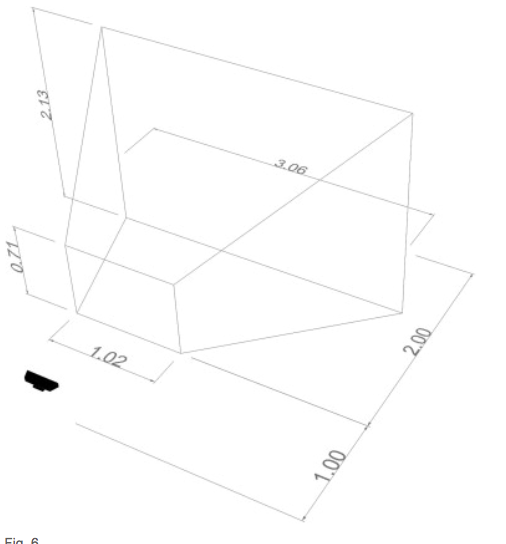
\includegraphics[width=0.5\textwidth]{figs/kinect_coverage}
\caption{The valid volume of a Kinect sensor~\cite{evaluation_kinect_workspace}}
\label{fig:kinect_coverage}
\end{figure}

\section{Posture Improvement Systems}
There have already been some techniques developed for posture improvement for the goods of human health. Lumo Back is one of the examples. It is a wearable sensor as the one developed to monitor seated spinal posture by Dunne et al.~\cite{wearable_spinal_posture}, attached on a belt to be worn on the user’s waist. It can detect slouch, and vibrate in response to the posture. In addition to the vibration feedback, it also passes the data via Bluetooth to the smartphone, and a specific application will illustrate current posture of user with the overall performance statistical pattern~\cite{review_lumo_posture_belt}. The device is light and the battery can last long. More importantly, the device is sensitive and multiple feedback can be provided~\cite{mindandmuscle_correct_posture}. However, according to Biggs~\cite{posture_saving_device}, the remainder of Lumo Back tends to lead users over-correct their postures, causing them to receive another wrong-posture feedback. Also, for users with poor postures, Lumo Back can be activated too often as well and get them annoyed.

Another technique developed for posture correction is a smartphone based real-time daily activity monitoring system. It will send a music-based alert when the system detects the user is about to fall down in order to remind them to correct their posture in time. Zhang et al.~\cite{smartphone_daily_activity_monitor} developed some algorithms for the system based on accelerometer, orientation principles and kinematical theory, for the use by different users in different environments. The judgment between a fall and a normal lying/sit-tilted is based on whether the music alarm is turned off in time~\cite{smartphone_daily_activity_monitor}. Several problems can be seen for the system. Firstly, many people may be not used to carry a smartphone by putting them in the pocket, or hold by hand all the time. Same problem will be even more apparent in the home setting. Few people tend to carry their smartphone by their bodies at home, where is the most common place for elderly, possibly the target users of the system. Secondly, the studies did not show whether feedback of the can effectively change the user's posture before they fall compared to the baseline measurement. Thirdly, the research did not run a user experience study to evaluate the usability of the system; therefore the user experience and other aspects of the system cannot be understood.

Another relevant technique to construct healthy postures is a monitor support apparatus. The monitor support apparatus is a reclining furniture, using special design to provide dorsal or ventral support for body. The design of the apparatus allows a range of adjustment. Pivots and telescopic joints are applied for the user to set a position and orientation facing the monitor. The user can find their preferred inclination of seat back on the apparatus in healthy postures without making extra effort~\cite{monitor_support_apparatus}. The apparatus will remain in the same configuration throughout an activity, thus supporting users healthy postures. However, the apparatus cannot actively construct healthy postural habit by providing users feedback on their current posture, which is a preferred method to improve users health because a habit for having healthy postures could be developed.

The three applications above all contribute to supporting healthy postures. However, the feedback of them can be more informative and a user study for its usability can be added to explore other aspects of the applications. These could be considered in the development of current posture improvement system.

\section{Feedback Techniques}
The feedback specification of the current system will be decided based on the analysis of previous studies and the findings from the following user study. The feedback will be delivered in multiple ways and through multiple perceptual channels. Using multiple feedback can reinforce the message to the user. Even though the user may miss or ignore some notifications, they will still have other ways to receive the same message. The feedback should also have different type that present different message. Previous studies have only one single feedback to all bad postures. However, the user may have no idea about which part of the body the problem comes from. Therefore, given a single mode of feedback, the user may have to employ the trial and error technique of adjusting different parts of the body until their posture is fixed, and they might not have enough patience.

The feedback should be delivered in a positive tone. According to Mind and Muscle~\cite{mindandmuscle_correct_posture}, it is important to provide feedback in a pleasant way that gives people receiving the signal a positive mood. In previous studies, a feedback is usually delivered to signal that the current posture or movement is not good, or even a threat to the user's health.This will easily create anxiety to the user and increase the threat level in the brain, which turns out to sensitize the central neuron system and results in higher possibility of chronic problems~\cite{mindandmuscle_correct_posture}. The fact is also explained by the Fear-Avoidance model~\cite{fear_avoidance_model_pain}. In short, the feedback should not create a sense that a user with a bad posture is in trouble, or should be blamed. Instead, it should try to make user believe that they are becoming healthier with the aid of the system.
